\documentclass[11pt]{article}

\usepackage[margin=1in]{geometry}
\usepackage{amsmath}
\usepackage{amssymb}
\usepackage{graphicx}

% monospace \texttt tokens cannot hyphenate; let TeX stretch a line rather than overflow
\emergencystretch=1em

\title{705.641.81: Homework 6}
\author{David Carrillo}
\date{}

\begin{document}
\maketitle

\section{Concepts, intuitions and big picture}

\begin{enumerate}
  \item How BERT expects a pair of sentences:
        \begin{itemize}
          \item[{[\ ]}] \texttt{Tokens-of-sentence-1 [SEP] Tokens-of-sentence-2}
          \item[{[\ ]}] \texttt{[CLS] Tokens-of-sentence-1 Tokens-of-sentence-2}
          \item[{[X]}] \texttt{[CLS] Tokens-of-sentence-1 [SEP] Tokens-of-sentence-2}
        \end{itemize}
        \texttt{[CLS]} is needed because its final hidden state is the pooled representation that sentence-pair
        heads read, and \texttt{[SEP]} is needed to mark where the first segment ends. None of the three options
        is quite the real format, which closes with a second \texttt{[SEP]} after the second segment and pairs
        the whole thing with a \texttt{token\_type\_ids} vector; the third is the only one with both special
        tokens in the right places.

  \item When to train a new tokenizer:
        \begin{itemize}
          \item[{[\ ]}] Dataset similar to an existing pretrained model's, and you want to pretrain a new model
          \item[{[\ ]}] Dataset similar to an existing pretrained model's, and you want to fine-tune using that
                pretrained model
          \item[{[X]}] Dataset different from the one used by an existing pretrained model, and you want to
                pretrain a new model
        \end{itemize}
        A tokenizer fixes the vocabulary, and the vocabulary fixes the number of rows in the embedding matrix,
        so a new tokenizer is incompatible with any existing checkpoint's weights. That rules out the
        fine-tuning option regardless of how different the data is. If the data resembles the pretraining
        corpus, the existing vocabulary already segments it well and a new one buys nothing.

  \item Statements that apply to BPE:
        \begin{itemize}
          \item[{[X]}] Starts with a small vocabulary and learns merge rules.
          \item[{[\ ]}] Starts with a big vocabulary and progressively removes tokens from it.
          \item[{[X]}] Learns merge rules by merging the pair of tokens that is the most frequent.
          \item[{[\ ]}] Learns a merge rule by merging the pair that maximizes a score privileging frequent
                pairs with less frequent individual parts.
          \item[{[X]}] Tokenizes words by splitting them into characters and then applying the merge rules.
          \item[{[\ ]}] Tokenizes words by finding the longest subword from the beginning that is in the
                vocabulary, then repeating for the rest.
        \end{itemize}
        The three rejected statements each describe a different algorithm. Pruning from a large vocabulary is
        Unigram, which starts oversized and removes the tokens whose loss contribution is smallest. The scoring
        rule that divides pair frequency by the frequencies of the individual parts is WordPiece, and that
        denominator is exactly what makes WordPiece prefer merges whose halves are rare on their own. Greedy
        longest-match from the start of the word is WordPiece's inference procedure, not BPE's. BPE replays its
        learned merges in the order it learned them, which is why its training and inference descriptions have
        to match.

  \item Labels in masked language modeling:
        \begin{itemize}
          \item[{[X]}] Tokens randomly masked, labels are the original input tokens.
          \item[{[\ ]}] Tokens randomly masked, labels are the original input tokens shifted to the left.
          \item[{[\ ]}] Tokens randomly masked, label is whether the sentence is positive or negative.
          \item[{[\ ]}] Tokens in two sentences randomly masked, label is whether the sentences are similar.
        \end{itemize}
        Shifting left is the causal objective, where position $t$ predicts token $t+1$. The point of masking is
        that the target is already in the input and gets hidden, so no shift is involved.

  \item When to pretrain a new model:
        \begin{itemize}
          \item[{[X]}] When there is no pretrained model available for your specific language
          \item[{[\ ]}] When you have lots of data available, even if there is a pretrained model that could
                work on it
          \item[{[X]}] When you have concerns about the bias of the pretrained model you are using
        \end{itemize}
        The middle option stipulates a pretrained model that could work on the data, and in that
        situation fine-tuning is cheaper and generally at least as accurate, so a large corpus is a
        precondition for pretraining and not a reason to choose it. The bias case is
        different in kind, because fine-tuning starts from the pretrained representation and inherits whatever
        is encoded in it, so no amount of task data fixes a tainted initialization.

  \item Whether the \texttt{bert-base-cased} tokenizer with the \texttt{gpt2} model is wrong:
        \begin{itemize}
          \item[{[\ ]}] No, it seems correct.
          \item[{[X]}] The tokenizer and model should always be from the same checkpoint.
          \item[{[\ ]}] It is good practice to pad and truncate with the tokenizer as every input is a batch.
        \end{itemize}
        The snippet does not fail. \texttt{bert-base-cased} encodes \texttt{"Hey!"} as ids \texttt{[101, 4403, 106, 102]}, every one of
        which is below GPT-2's vocabulary size of 50257, so the embedding lookup stays in bounds and the forward
        pass returns a well-formed $1 \times 4 \times 768$ tensor with no exception. The ids simply mean
        something else in the other vocabulary: id 4403 is the subword \texttt{\.{G}Big} to GPT-2 rather than
        \texttt{Hey}, and the three remaining ids land on stray byte-level fragments, since GPT-2 has no
        \texttt{[CLS]} or \texttt{[SEP]} at all and those two sentinel positions become noise rather than
        structure. GPT-2's own encoding of the same string is \texttt{[10814, 0]}, two tokens rather than four. A silent
        wrong answer is worse than a crash here, which is why the rule is stated as absolute.
\end{enumerate}

\section{Getting Your Attention with Self-Attention}

\subsection*{2.1 Forget `Softmax', `Argmax' is the New Boss in Town!}

\begin{enumerate}
  \item The argmax runs over the query-key inner products, so only those four scalars matter:
        \[
          \mathbf{q}^{\top}\mathbf{k}_1 = 0 + 1 + 2 = 3, \qquad
          \mathbf{q}^{\top}\mathbf{k}_2 = -2 + 1 + 2 = 1,
        \]
        \[
          \mathbf{q}^{\top}\mathbf{k}_3 = 2 + 1 - 2 = 1, \qquad
          \mathbf{q}^{\top}\mathbf{k}_4 = 0 - 1 - 2 = -3 .
        \]
        The scores are $[3, 1, 1, -3]$, so $\operatorname{argmax} = [1, 0, 0, 0]$ and the layer returns the
        first value vector,
        \[
          \text{Attention}(\mathbf{q}, \mathbf{K}, \mathbf{V}) = \mathbf{v}_1
          = \begin{bmatrix} 3 & 2 & -4 \end{bmatrix}^{\top} .
        \]
        The maximum is strict, but positions 2 and 3 tie at 1, so a query only slightly different could land
        on a tie where the argmax is undefined.

  \item The attention weights become a piecewise constant function of the scores. Within the region where
        $\mathbf{k}_1$ wins, perturbing $\mathbf{q}$ or any $\mathbf{k}_i$ leaves the output exactly at
        $\mathbf{v}_1$, so $\partial \text{Attention} / \partial \mathbf{q} = \mathbf{0}$ and
        $\partial \text{Attention} / \partial \mathbf{k}_i = \mathbf{0}$ everywhere except on the tie
        boundaries, where the output jumps and the derivative does not exist. Training therefore gets no signal
        into $\mathbf{W}_q$ or $\mathbf{W}_k$: the queries and keys cannot be improved, because the loss cannot
        tell the difference between a query that barely wins and one that wins by a mile. The only surviving
        gradient path is through the selected value, so $\mathbf{W}_v$ learns, and even then only from the one
        position that was chosen while the other $n-1$ value vectors receive nothing. Softmax is what makes the
        layer trainable rather than merely evaluable, since every weight is a differentiable function of every
        score and so each key and query gets a share of the gradient.
\end{enumerate}

\subsection*{2.2 Superposition of Information in Self-Attention}

\begin{enumerate}
  \item The output is the convex combination $\sum_{t'} \alpha^{(t)}_{t'} \mathbf{v}_{t'}$, so it collapses onto
        $\mathbf{v}_j$ exactly when $\alpha^{(t)}_j$ absorbs nearly all the mass, which happens when
        $\mathbf{q}_t$ is far more aligned with $\mathbf{k}_j$ than with any other key, meaning
        $\mathbf{q}_t^{\top}\mathbf{k}_j - \max_{i \neq j} \mathbf{q}_t^{\top}\mathbf{k}_i \gg \sqrt{h}$.
        Scaling $\mathbf{q}_t$ up in the direction of $\mathbf{k}_j$ achieves this on its own, since the margin
        grows with $\|\mathbf{q}_t\|$ while the number of competing keys does not.

  \item Collect the basis of $A$ as the columns of $\mathbf{A} = [\mathbf{a}_1 \ \cdots \ \mathbf{a}_m]$ and take
        \[
          \mathbf{M} = 2\mathbf{A}\mathbf{A}^{\top} = 2\sum_{j=1}^{m} \mathbf{a}_j \mathbf{a}_j^{\top}.
        \]
        $\mathbf{A}\mathbf{A}^{\top}$ is the orthogonal projector onto $A$, which is what the two stated
        properties buy. Writing $\mathbf{v}_a = \sum_j c_j \mathbf{a}_j$, orthonormality of the basis gives
        $\mathbf{A}^{\top}\mathbf{v}_a = \mathbf{c}$ and hence
        $\mathbf{A}\mathbf{A}^{\top}\mathbf{v}_a = \mathbf{A}\mathbf{c} = \mathbf{v}_a$, while orthogonality of
        the two subspaces gives $\mathbf{a}_j^{\top}\mathbf{v}_b = 0$ for every $j$ and hence
        $\mathbf{A}\mathbf{A}^{\top}\mathbf{v}_b = \mathbf{0}$. Therefore
        \[
          \mathbf{M}\bar{\mathbf{v}}
          = 2\mathbf{A}\mathbf{A}^{\top}\cdot \tfrac{1}{2}(\mathbf{v}_a + \mathbf{v}_b)
          = \mathbf{A}\mathbf{A}^{\top}\mathbf{v}_a + \mathbf{A}\mathbf{A}^{\top}\mathbf{v}_b
          = \mathbf{v}_a + \mathbf{0} = \mathbf{v}_a,
        \]
        for arbitrary $\mathbf{v}_a \in A$ and $\mathbf{v}_b \in B$. The factor of 2 only undoes the averaging;
        the projector does the actual separation. Nothing here uses the basis of $B$, which is why $p$ never
        appears in $\mathbf{M}$.

  \item Take $\mathbf{q}_t = c\sqrt{h}\,(\mathbf{k}_a + \mathbf{k}_b)$ for a large positive constant $c$. The
        keys are orthonormal, so the scaled scores are
        \[
          \frac{\mathbf{q}_t^{\top}\mathbf{k}_a}{\sqrt{h}} = c, \qquad
          \frac{\mathbf{q}_t^{\top}\mathbf{k}_b}{\sqrt{h}} = c, \qquad
          \frac{\mathbf{q}_t^{\top}\mathbf{k}_i}{\sqrt{h}} = 0 \quad (i \neq a, b),
        \]
        giving $\alpha_a = \alpha_b = e^{c} / (2e^{c} + n - 2)$ and the same denominator with numerator 1 for
        each of the other $n-2$ positions. As $c$ grows, $\alpha_a$ and $\alpha_b$ both approach $\tfrac{1}{2}$
        and the rest vanish geometrically, so the output approaches
        $\tfrac{1}{2}(\mathbf{v}_a + \mathbf{v}_b)$. The equality is exact only in the limit. The $\sqrt{h}$ cancels, leaving
        $\alpha_a = 1/(2 + (n-2)e^{-c})$, so with $n = 6$ and $c = 20$ both weights are within
        $10^{-8}$ of a half; the output is within $10^{-8}$ of the target when the value vectors have
        norm of order one, which the problem leaves unstated. At $c = 1$ there is a visible
        error. Symmetry between $\mathbf{k}_a$ and $\mathbf{k}_b$ forces the two weights to be equal; the
        magnitude $c$ suppresses everything else.
\end{enumerate}

\subsection*{2.3 Extra Credit: Importance of `Scaling' in Self-Attention}

With $\mathbf{q}, \mathbf{k} \in \mathbb{R}^{1 \times h}$ drawn independently from
$\mathcal{N}(\mu, \sigma^2 \mathbf{I})$, the dot product is the scalar
$\mathbf{q}\mathbf{k}^{\top} = \sum_{i=1}^{h} q_i k_i$, and all $2h$ components are mutually independent.

\begin{enumerate}
  \item Independence splits each term, so
        \[
          \mathbb{E}[\mathbf{q}\mathbf{k}^{\top}] = \sum_{i=1}^{h} \mathbb{E}[q_i k_i]
          = \sum_{i=1}^{h} \mathbb{E}[q_i]\,\mathbb{E}[k_i] = h\mu^2 .
        \]

  \item The $h$ products $q_i k_i$ are independent of each other, so their variances add. For one of them,
        \[
          \operatorname{Var}[q_i k_i] = \mathbb{E}[q_i^2 k_i^2] - \big(\mathbb{E}[q_i k_i]\big)^2
          = \mathbb{E}[q_i^2]\,\mathbb{E}[k_i^2] - \mu^4
          = (\sigma^2 + \mu^2)^2 - \mu^4 = \sigma^4 + 2\sigma^2\mu^2 ,
        \]
        using $\mathbb{E}[q_i^2] = \sigma^2 + \mu^2$. Summing over $i$,
        \[
          \operatorname{Var}[\mathbf{q}\mathbf{k}^{\top}] = h\big(\sigma^4 + 2\sigma^2\mu^2\big)
          = h\sigma^2\big(\sigma^2 + 2\mu^2\big) .
        \]

  \item Setting $\mu = 0$ and $\sigma = 1$ leaves $\mathbb{E}[\mathbf{q}\mathbf{k}^{\top}] = 0$ and
        $\operatorname{Var}[\mathbf{q}\mathbf{k}^{\top}] = h$, so the standard deviation of an unscaled score is
        $\sqrt{h}$ and grows with the hidden dimension. Dividing by $\sqrt{h}$ returns the scores to unit
        variance for every $h$, which makes the softmax input distribution independent of model width.

        Numerical stability is the consequence. For a 64-dimensional head the unscaled scores have standard
        deviation 8, so the largest and smallest logits in a row routinely sit tens of units apart; softmax of
        such a row is nearly one-hot. That hurts in both directions. The Jacobian of the softmax at output
        $\hat{\mathbf{y}}$ has entries $\hat{y}_i(\delta_{ij} - \hat{y}_j)$, which go to zero as the
        distribution saturates, so the gradient reaching the queries and keys dies exactly when the scores get
        large. A stabilized softmax subtracts the row maximum before exponentiating, so overflow is not the
        practical failure; saturation is. Scaling keeps the scores order one and the softmax in the
        regime where it still has a usable derivative.
\end{enumerate}

\section{Programming}

BoolQ's validation split answers yes on 2{,}033 of 3{,}270 questions, so a classifier that
ignores its input and always answers yes scores $0.6217$ on that split. Dev accuracies below are measured against
it. The test split is \texttt{train[8000:]} from an unseeded shuffle, so its own majority rate
differs from run to run.

\subsection*{3.1 Finetuning: Basics}

\begin{enumerate}
  \item \texttt{load\_dataset("boolq")} no longer resolves, because current \texttt{datasets}
        requires a namespaced repository id; the call is \texttt{load\_dataset("google/boolq")}
        throughout. Training accuracy on the ten-instance subset rises from $0.40$ to $1.00$ and
        first reaches $1.00$ at epoch 16, so the implementation can memorize its training data.
        \begin{center}
          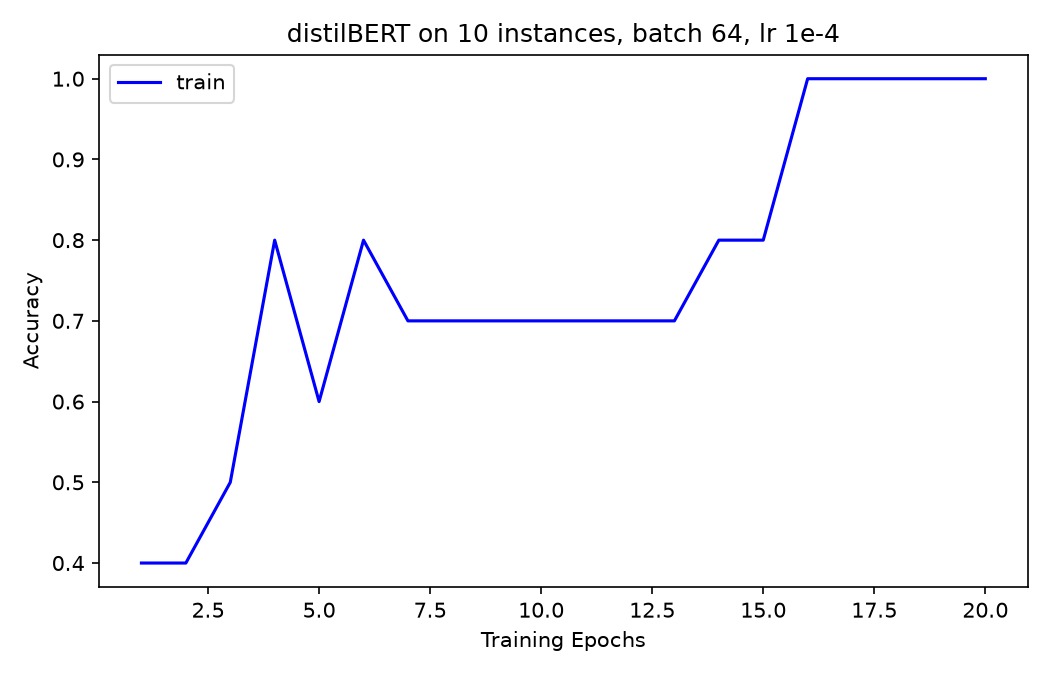
\includegraphics[width=0.62\textwidth]{figs/fig_3_1_1_overfit.png}
        \end{center}

  \item Largest batch size: \textbf{778}. Measured by doubling the batch until a full AdamW step raised \texttt{OutOfMemoryError} and
        then bisecting. A parameter count would not predict it, because the optimizer's two moment
        tensors per parameter are what exhaust the card. At 778 the peak allocation is 29.79 GB of 31.4 GB available.
        The 30-epoch run below uses batch 32, which keeps it comparable with the sweeps that
        follow.

        \begin{center}
          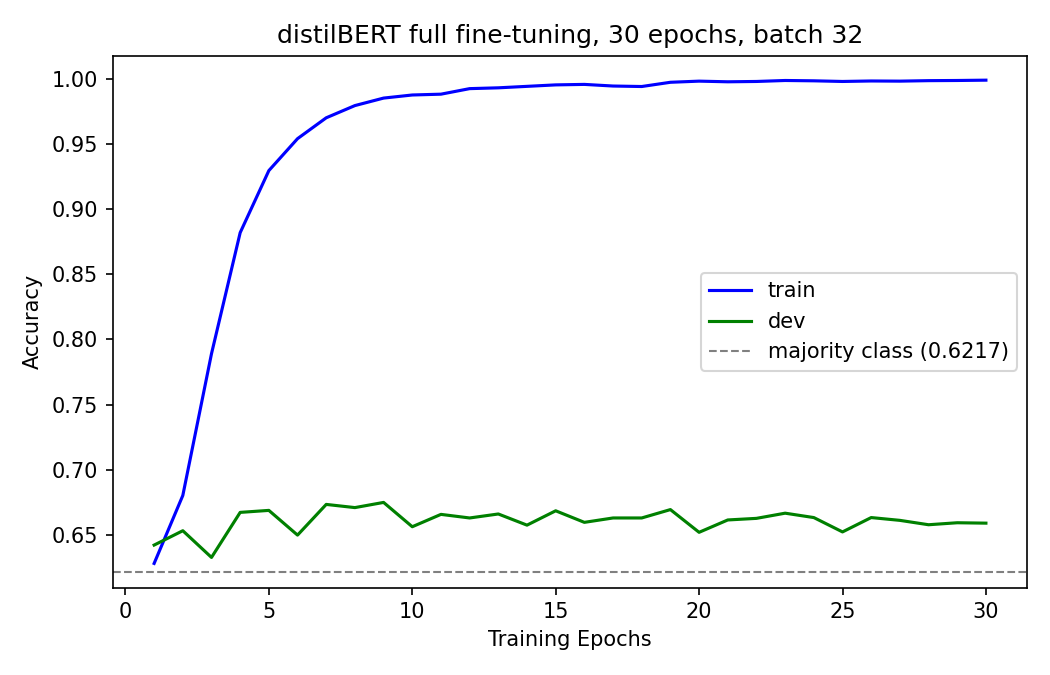
\includegraphics[width=0.72\textwidth]{figs/fig_3_1_2_full30.png}
        \end{center}

        Training accuracy climbs from $0.6281$ to $0.9989$ and validation accuracy ends at
        $0.6590$, a gap of $0.3399$. The handout predicts that dev accuracy will rise and then
        turn downhill, and only the first half of that happens here. Dev reaches $0.6749$ at epoch 9 and then stays between $0.6520$ and $0.6694$ for the
        remaining twenty-one epochs; the $0.0159$ drop from that peak to its final value is smaller
        than the $0.0174$ width of that band, so it is noise rather than a trend. The memorization is unambiguous and the degradation is not, so the train/dev gap is the
        evidence of overfitting rather than any decline in the dev curve.

  \item Six configurations, three learning rates by two epoch counts:

        \begin{center}
        \begin{tabular}{|l|r|r|r|}
          \hline
          Learning rate & Epochs & Dev accuracy & Test accuracy \\
          \hline
          $1 \times 10^{-4}$ & 7 & \textbf{0.6936} & \textbf{0.6819} \\
          $1 \times 10^{-4}$ & 9 & 0.6566 & 0.6510 \\
          $5 \times 10^{-4}$ & 7 & 0.6217 & 0.6426 \\
          $5 \times 10^{-4}$ & 9 & 0.6217 & 0.6279 \\
          $1 \times 10^{-3}$ & 7 & 0.6217 & 0.6132 \\
          $1 \times 10^{-3}$ & 9 & 0.6217 & 0.6027 \\
          \hline
        \end{tabular}
        \end{center}

        The best model on dev uses $\mathbf{lr} = 1 \times 10^{-4}$ for \textbf{7 epochs} and
        scores \textbf{0.6819 on test}.

        Four of the six rows read $0.6217$, and not as a rounded coincidence: those runs report dev accuracy of $0.6217125382262997$, which is
        $2033/3270$ to the last digit of double precision. Their training accuracy flattens too, each at its own slice's majority rate: $0.619625$,
        $0.62225$, $0.624875$ and $0.62675$. Those four differ because \texttt{dataset.shuffle()}
        is unseeded, so every run draws a different \texttt{train[:8000]}. At
        $5 \times 10^{-4}$ and above the model collapses onto the constant prediction and never
        leaves it, so the sweep separates two models that learned from four that did not.

        One caveat on the test column. \texttt{pre\_process} calls
        \texttt{dataset.shuffle()} with no seed, and the test split is \texttt{train[8000:]}, so
        each run draws its 1{,}427 test instances from a different shuffle. The dev column is
        comparable across rows because the validation split's membership is fixed and only its
        order changes, but the test figures carry that extra variance.

  \item Repeating the sweep on \texttt{bert-base-uncased} and \texttt{roberta-large}:

        \begin{center}
          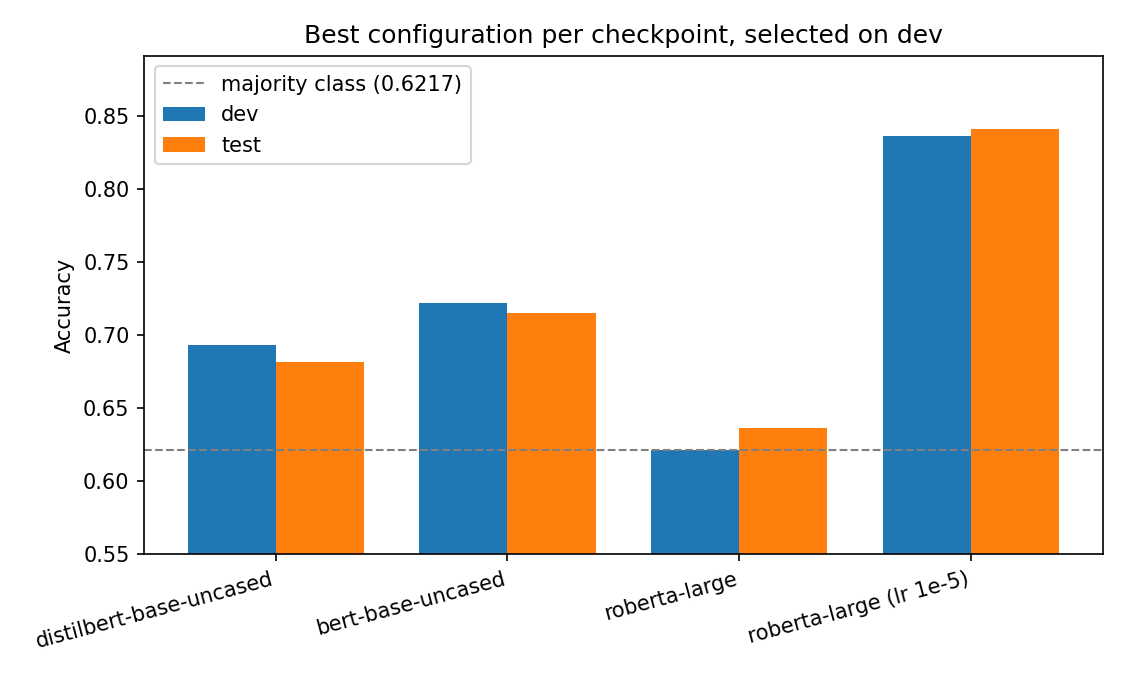
\includegraphics[width=0.78\textwidth]{figs/fig_3_1_4_models.png}
        \end{center}

        \texttt{bert-base-uncased} is the better of the two prescribed checkpoints at
        $0.7217$ dev and $0.7148$ test, again at $1 \times 10^{-4}$ for 7 epochs, and again with
        four of its six configurations collapsed.

        \texttt{roberta-large} collapsed in all six. Its final dev accuracy is $0.6217$ at every learning rate and epoch count. Five of the six sit
        there from the first epoch; at $1 \times 10^{-3}$ for 9 epochs the model instead alternated
        between $0.3783$ and $0.6217$ for four epochs before settling, which are the all-no and
        all-yes constant predictions ($1237/3270$ and $2033/3270$). The handout offers reporting zero for a checkpoint that will not fit, but that
        is not what happened: it fits comfortably, with a largest trainable batch of 137, so this
        is a learning-rate failure and not a memory one. Every rate in the prescribed grid is
        above the usable range for a 355M-parameter encoder, where $1$ to $2 \times 10^{-5}$ is
        the conventional choice.

        One configuration outside the grid tests that reading, and it holds:
        \texttt{roberta-large} at $1 \times 10^{-5}$ for 7 epochs reaches \textbf{0.8361 dev and
        0.8409 test}, with training accuracy moving $0.6733 \rightarrow 0.9804$. That is the
        strongest result anywhere in this assignment, 11 points above
        \texttt{bert-base-uncased} and 21 above the majority baseline. The grid hides the best model on the list.
\end{enumerate}

\subsection*{3.2 Parameter-Efficient Fine-Tuning}

{\sloppy
Three defects in the provided code have to be fixed, and none of them stops \texttt{type="full"}
from running; they break head- and prefix-tuning only. First, the hints for the head and prefix
optimizers say to call \texttt{mymodel.head.parameters()}, but \texttt{\_\_init\_\_} builds the
layer as \texttt{self.classifier} and no \texttt{head} attribute exists, so following the hint
raises \texttt{AttributeError}; the call is \texttt{mymodel.classifier.parameters()}. Second,
\texttt{get\_scheduler} was given \texttt{optimizer} while the training loop steps
\texttt{custom\_optimizer} for head- and prefix-tuning, so the scheduler was mutating the learning
rate of an optimizer that is never stepped; left alone, those two methods would train at a
constant rate with no warmup and no decay. It is now bound to whichever optimizer the loop steps.
Third, the skeleton builds the prefix \texttt{Parameter} in every mode and pins it to
\texttt{cuda} at construction. Built unconditionally it sits in \texttt{named\_parameters()} for
head-tuning too, unused and never given a gradient, which would add $128 \times 768$ to the counts
reported below; it is now created only for \texttt{type="prefix"}.
\par}

The handout prescribes the averaged token representation. The skeleton pads every input to
\texttt{max\_len = 128}, so that mean runs over padding as well. On short inputs most of
those positions are \texttt{<pad>}, so the signal is diluted and a mask-weighted mean would be the
better estimator.

The provided tokenization changes meaning once the backbone changes. The dataset class joins question and passage with the literal string \texttt{" [SEP] "}, which is a
real token for the BERT family. RoBERTa's separator is \texttt{</s>} and \texttt{[SEP]} is not in
its vocabulary at all, so for every example in this subsection that separator is encoded as the
four subwords \texttt{[}, \texttt{SE}, \texttt{P}, \texttt{]}. The model still learns, but it is
learning to read a four-token artefact as a field boundary rather than being given one.

\begin{enumerate}
  \item \textbf{Full fine-tuning, RoBERTa-base.} Learning rate $1 \times 10^{-5}$, 7 epochs,
        batch 32: \textbf{dev 0.7740, test 0.7779}. I chose $10^{-5}$ rather than anything from
        3.1.3's grid because that sweep showed every rate at $10^{-4}$ and above collapsing
        encoders of this size onto the majority class, and RoBERTa-base at 125M parameters sits
        closer to \texttt{roberta-large} than to distilBERT.

  \item Head-tuning. Tuned parameters $2d + 2$, which is \textbf{1{,}538} at $d = 768$. The classifier is a single $d \times 2$ linear layer plus its two biases, and
        nothing else receives a gradient.

        At $1 \times 10^{-3}$ for 10 epochs: dev 0.6431, test 0.6272. The handout's footnote
        suggests a larger rate and longer training, so a second run used $5 \times 10^{-3}$ for 20
        epochs: \textbf{dev 0.6532, test 0.6510}. The hint helps by about one point of dev
        accuracy and the result is still only three points above the $0.6217$ baseline, which is
        what 1{,}538 parameters on a frozen encoder can buy.

  \item Prefix-tuning. Tuned parameters $128d + 2d + 2 = 130d + 2$, which is \textbf{99{,}842} at $d = 768$: the prefix contributes $128 \times 768 = 98{,}304$ and
        the classification head the same $1{,}538$ as above, since prefix-tuning trains the head
        too.

        At $1 \times 10^{-3}$ for 10 epochs: dev 0.6309, test 0.6370. At $5 \times 10^{-3}$ for
        20 epochs: \textbf{dev 0.6572, test 0.6629}. Prefix-tuning gains more from the longer
        schedule than head-tuning does, $+0.0263$ against $+0.0101$ on dev, which is consistent
        with it having 65 times more parameters to move.

  \item \textbf{Extra credit: memory.} Measured on one RTX 5090 at batch 32 and sequence length
        128. The forward column is peak allocation during the forward pass. The backward column is
        the \emph{additional} peak on top of the live forward activations, since the counter is
        reset between the two, which is why it is much the smaller number. The handout points at
        \texttt{torch.profile}; its per-scope CUDA attribution returned $0.0$ for all three
        methods, so these figures come from \texttt{torch.cuda.max\_memory\_allocated}.

        \begin{center}
          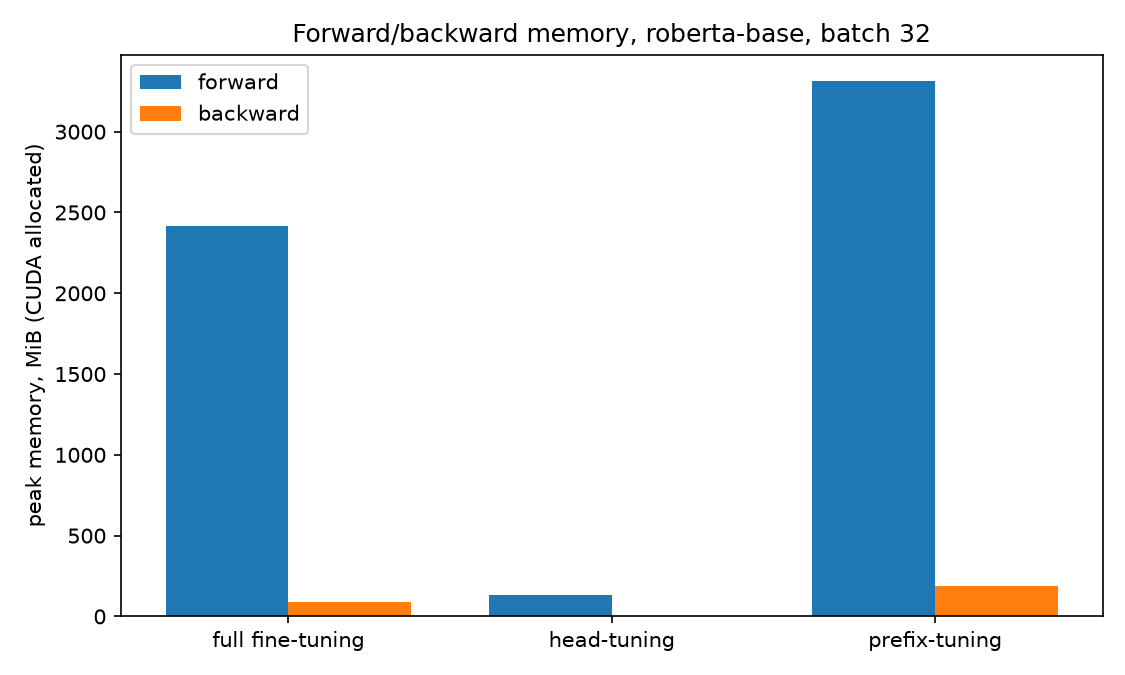
\includegraphics[width=0.72\textwidth]{figs/fig_3_2_4_memory.png}
        \end{center}

        \begin{center}
        \begin{tabular}{|l|r|r|r|}
          \hline
          Method & Trainable parameters & Forward (MiB) & Backward (MiB) \\
          \hline
          Full fine-tuning & 124{,}647{,}170 & 2418.1 & 89.9 \\
          Head-tuning      & 1{,}538         & 132.0  & 0.0   \\
          Prefix-tuning    & 99{,}842        & 3312.2 & 185.8 \\
          \hline
        \end{tabular}
        \end{center}

        Prefix-tuning costs \emph{more} forward memory than full fine-tuning, 3312 MiB against 2418, while
        training $0.08\%$ of the parameters. Two
        effects compound. The 128-token prefix doubles the sequence from 128 to 256, and
        attention memory grows with the square of that. The prefix is also a leaf tensor requiring gradient and it enters at the very bottom of the network, so reaching it
        in the backward pass requires the activations of every layer above it. Freezing the
        encoder's weights stops them from being updated but does not stop their activations from
        being stored.

        Head-tuning is the only one of the three that is cheap, at $132$ MiB forward and
        an immeasurably small backward, because the gradient stops at the classifier and nothing
        upstream has to be retained.

        The Module 7 lecture on parameter-efficient fine-tuning asks whether these methods are
        more computationally and more memory efficient than whole-model tuning, and answers that
        they are not faster, since the full forward and backward pass still runs, but that they
        are more memory efficient because only the tuned parameters need optimizer state. Both
        halves of that hold here, and the figures above do not contradict it: this measurement
        builds no optimizer at all, so it captures activations and gradients rather than the
        optimizer state the lecture is talking about. On that axis the saving is real and large,
        since AdamW keeps two moment tensors per trainable parameter, which is 99{,}842 of them
        for prefix-tuning against 124{,}647{,}170 for full fine-tuning.

        The saving does not extend to activation memory, which scales with where the tuned parameter
        sits and how long the sequence is, and for prefix-tuning it reverses.

  \item \textbf{LoRA storage.} With $\Delta M \approx AB$ for $A \in \mathbb{R}^{d \times n}$ and
        $B \in \mathbb{R}^{n \times d}$, gradients and optimizer states are needed for
        $dn + nd = \mathbf{2nd}$ parameters per adapted matrix, against $d^2$ for the full
        update. At $d = 768$ and $n = 8$ that is $12{,}288$ rather than $589{,}824$, a factor of
        48.

  \item \textbf{Extra credit: LoRA.} \texttt{classification\_lora.py} is
        \texttt{base\_classification.py} with the \texttt{peft} wrapper added, applied to the
        \texttt{query} and \texttt{value} projections with \texttt{task\_type=SEQ\_CLS},
        \texttt{r=8}, \texttt{lora\_alpha=16} and \texttt{lora\_dropout=0.1}. Learning rate
        $5 \times 10^{-4}$, 7 epochs, batch 32.

        Trainable parameters \textbf{887{,}042} of 125{,}534{,}212, or $0.7066\%$.
        Dev \textbf{0.7639}, test \textbf{0.7589}.

        LoRA reaches $0.7639$ dev against full fine-tuning's $0.7740$ and head- and prefix-tuning's
        $0.6532$ and $0.6572$, while updating about one parameter in 142. {\sloppy Two things stop that from
        being a clean comparison. The $887{,}042$ is not mostly adapters: the rank-8 updates on
        \texttt{query} and \texttt{value} across 12 layers come to $294{,}912$, and the remaining
        $592{,}130$ is RoBERTa's own classification head, which
        \texttt{AutoModelForSequenceClassification} builds as a $768 \times 768$ dense layer plus a
        $768 \times 2$ projection. That head also reads the \texttt{<s>} token rather than the
        padding-diluted mean the other three methods use, and this run used
        $5 \times 10^{-4}$ where full fine-tuning used $1 \times 10^{-5}$. So the 11-point margin
        over head- and prefix-tuning is not attributable to the adapters alone; pooling, head
        capacity and learning rate all differ. What the adapters do add is the ability to change the
        encoder's representations at all, which head- and prefix-tuning cannot do.\par}

        \texttt{task\_type=SEQ\_CLS} keeps the freshly initialized classification head trainable alongside the adapters; without it the head
        would be frozen with the rest of the backbone, and it has no pretrained weights to adapt.
\end{enumerate}

\subsection*{3.3 In-Context Learning}

{\sloppy
The models this subsection requires, \texttt{gpt-3.5-turbo-instruct} and \texttt{davinci}, are deprecated and no longer callable.
I raised this by email and was told to skip them.
\par}

\end{document}
